\section{Introduction}

Since its discovery, the Dunhuang Grottoes have been an important site for the study of Buddhist art and
several important aspects of Chinese history, including the trade events via the Silk Road, etc.
While a large quantity of artefacts like the murals and sculptures have survived thousands of years
to be presented in this modern age, the artefacts are facing significant threats from various factors.
A study of \apaciteassub{Jiang2023-Weather-Dunhuang} has shown that the despite the lack of immediate risk
of preservation due to the drastic climate change in the past few decades, the artefacts are still
prone to deterioration due to the weathering effects of the natural environment. Therefore, the
preservation of the Dunhuang treasures is of utmost importance and a race against time
(\apaciteaspar{Yu2022-AI-Dunhuang}). Measures with high efficiency are needed to ensure the survival
of the cultural heritage.

In view of the above, the Dunhuang Research Academy (DHA) was established in 1944 and is now devoted to
applying modern technologies to the preservation of the Dunhuang Grottoes. While one takes advantage of
the efficiency and convenience of modern technologies, such as Artificial Intelligence (AI), one must
also be careful about the potential damages that may be imposed on the cultural heritage.
This essay aims to explore the current applications of the AI technology in the preservation of the 
Buddhist heritage, using the Dunhuang Caves as a case study. In the Literature Review section, some
cutting-edge AI applications in the archaeological field will be briefly explored. Then, in the
following two sections, the benefits and potential risks of these applications will be discussed.
Finally, a conclusion on the topic will be included, with a hope that the discussion would provide new
insights into the process of critically evaluating the use of AI in the preservation of cultural heritage.

\subsection{Terminology}

Since the topics ``cultural heritage'', ``preservation'' and ``AI'' are all broad, it may be helpful if
these terms are defined before the discussion commences. 

\subsubsection{Buddhist Heritage and Cultural Heritage}

In the context and the scope of discussion of this essay, the term ``Buddhist heritage'' and ``cultural
heritage'' are treated as the same, and they refer to both the artefacts and sites of the Dunhuang Grottoes.
The ``artefacts'' include the mural paintings, sculptures, manuscripts that were recovered from the Library
Cave (Cave 17) and other caves. The ``sites'' refer to the region, and the caves' architectural and structural
designs and features. This definition is consistent with that of the current standard as suggested by
\apaciteassub{UNESCO2024-Cultural-Heritage}.

\subsubsection{Preservation}

As suggested by \apaciteassub{UNESCO2024-Conservation}, the conservation and preservation of cultural heritage
are means taken to elongate the lifespan of the heritage and to convey its significance to the future
generations. Therefore, the term ``preservation'' would imply two aspects: the technical aspect of 
protecting the existence of the artefacts and sites, and the human aspect of public education and raising
awareness.

\subsubsection{Artificial Intelligence}

Contrary to the common generic definition of AI as ``the simple theory of human intelligence being
exhibited by machines'' (\apaciteaspar{Helm2020-AI-Orthopedics}, p. 69), this essay will refer to AI simply
as a set of tools utilising Machine Learning (ML), Convolutional Neural Networks (CNNs), Large
Language Models (LLMs), and Natural Language Processing (NLP) technologies
dedicated to the analysis and processing of images and texts for the purpose of
preserving cultural heritage.

\section{Literature Review}

Current AI applications in the study and preservation of Dunhuang Grottoes can be roughly categorised into
image-related techniques and text-related techniques.

\subsection{Computer Vision and Image Processing}

Algorithms specialised in computer vision and image processing, such as CNNs, Revolutional Neural Networks
(RNNs), and Generative Adversarial Networks (GANs), and hybrids of these algorithms are most prominently
used in the handling the murals of the Dunhuang Grottoes (\apaciteaspar{Fu2025-AI-Intangible-Cultural-Heritage};
\apaciteaspar{Yu2022-AI-Dunhuang}).

For the restoration of damaged murals, conventional patch-based methods
(\apasecciteaspar{Ballester et al.}{2001}{Yu2022-AI-Dunhuang}; \apasecciteaspar{Bertalmio}{2000}{Yu2022-AI-Dunhuang})
allowed automatic inpainting of small and simple damaged areas. Their inability to handle larger and more complex
missing areas have been overcome by modern use of CNNs (\apasecciteaspar{Pathak et al.}{2016}{Yu2022-AI-Dunhuang};
\apasecciteaspar{Yang et al.}{2017}{Yu2022-AI-Dunhuang}).
In recent years, \apasecciteassub{Song et al.}{2018}{Yu2022-AI-Dunhuang} proposed a more modern approach,
allowing the restoration and inpainting be context-aware, i.e. the algorithm would reconstruct the missing parts
by considering the surrounding context, rather than simply predicting pixels mathematically.
Similar means include systems built on CNNs and the ResNet-50 architecture, which are employed by the British
Museum and Le Musée du Louvre (the Louvre Museum) for damage recognition
(\apaciteaspar{Fu2025-AI-Intangible-Cultural-Heritage}).
Recent studies carried out by \apaciteassub{Chen2024-Mural-Inpainting} proposed a hybrid approach of joint
learning, further improving the errors produced by the AI models by allowing the models to learn from the global
context of the murals, rather than just the local context.

For creating arts in the visual style of the Dunhuang murals through AI, specialised algorithms referred to as
the ``style transfer'' algorithms are used (\apaciteaspar{Sun2023-Dunhuang-Patterns};
\apaciteaspar{Yu2022-AI-Dunhuang}). While \apaciteassub{Yu2022-AI-Dunhuang} mentioned certain limitations of the
algorithms built on the CNNs, such as lack of flexibility and optimisation, an experiment carried out by 
\apaciteaspar{Sun2023-Dunhuang-Patterns}, as shown in Figure \ref{fig:style-transfer-showcase}
displayed satisfactory results in transferring
the visual styles of the Dunhuang murals from different dynasties onto modern images.
Apart from application on Dunhuang murals,
a recent study by \apaciteassub{Zhang2023-AI-New-Year-Prints} also mentioned advanced techniques for generating
cultural and creative products by replicating visual styles from the input.

\begin{figure}
    \caption{Examples of results of merging Dunhuang art styles with modern images using different 
    models and algorithms.}
    \label{fig:style-transfer-showcase}
    
    \begin{center}
        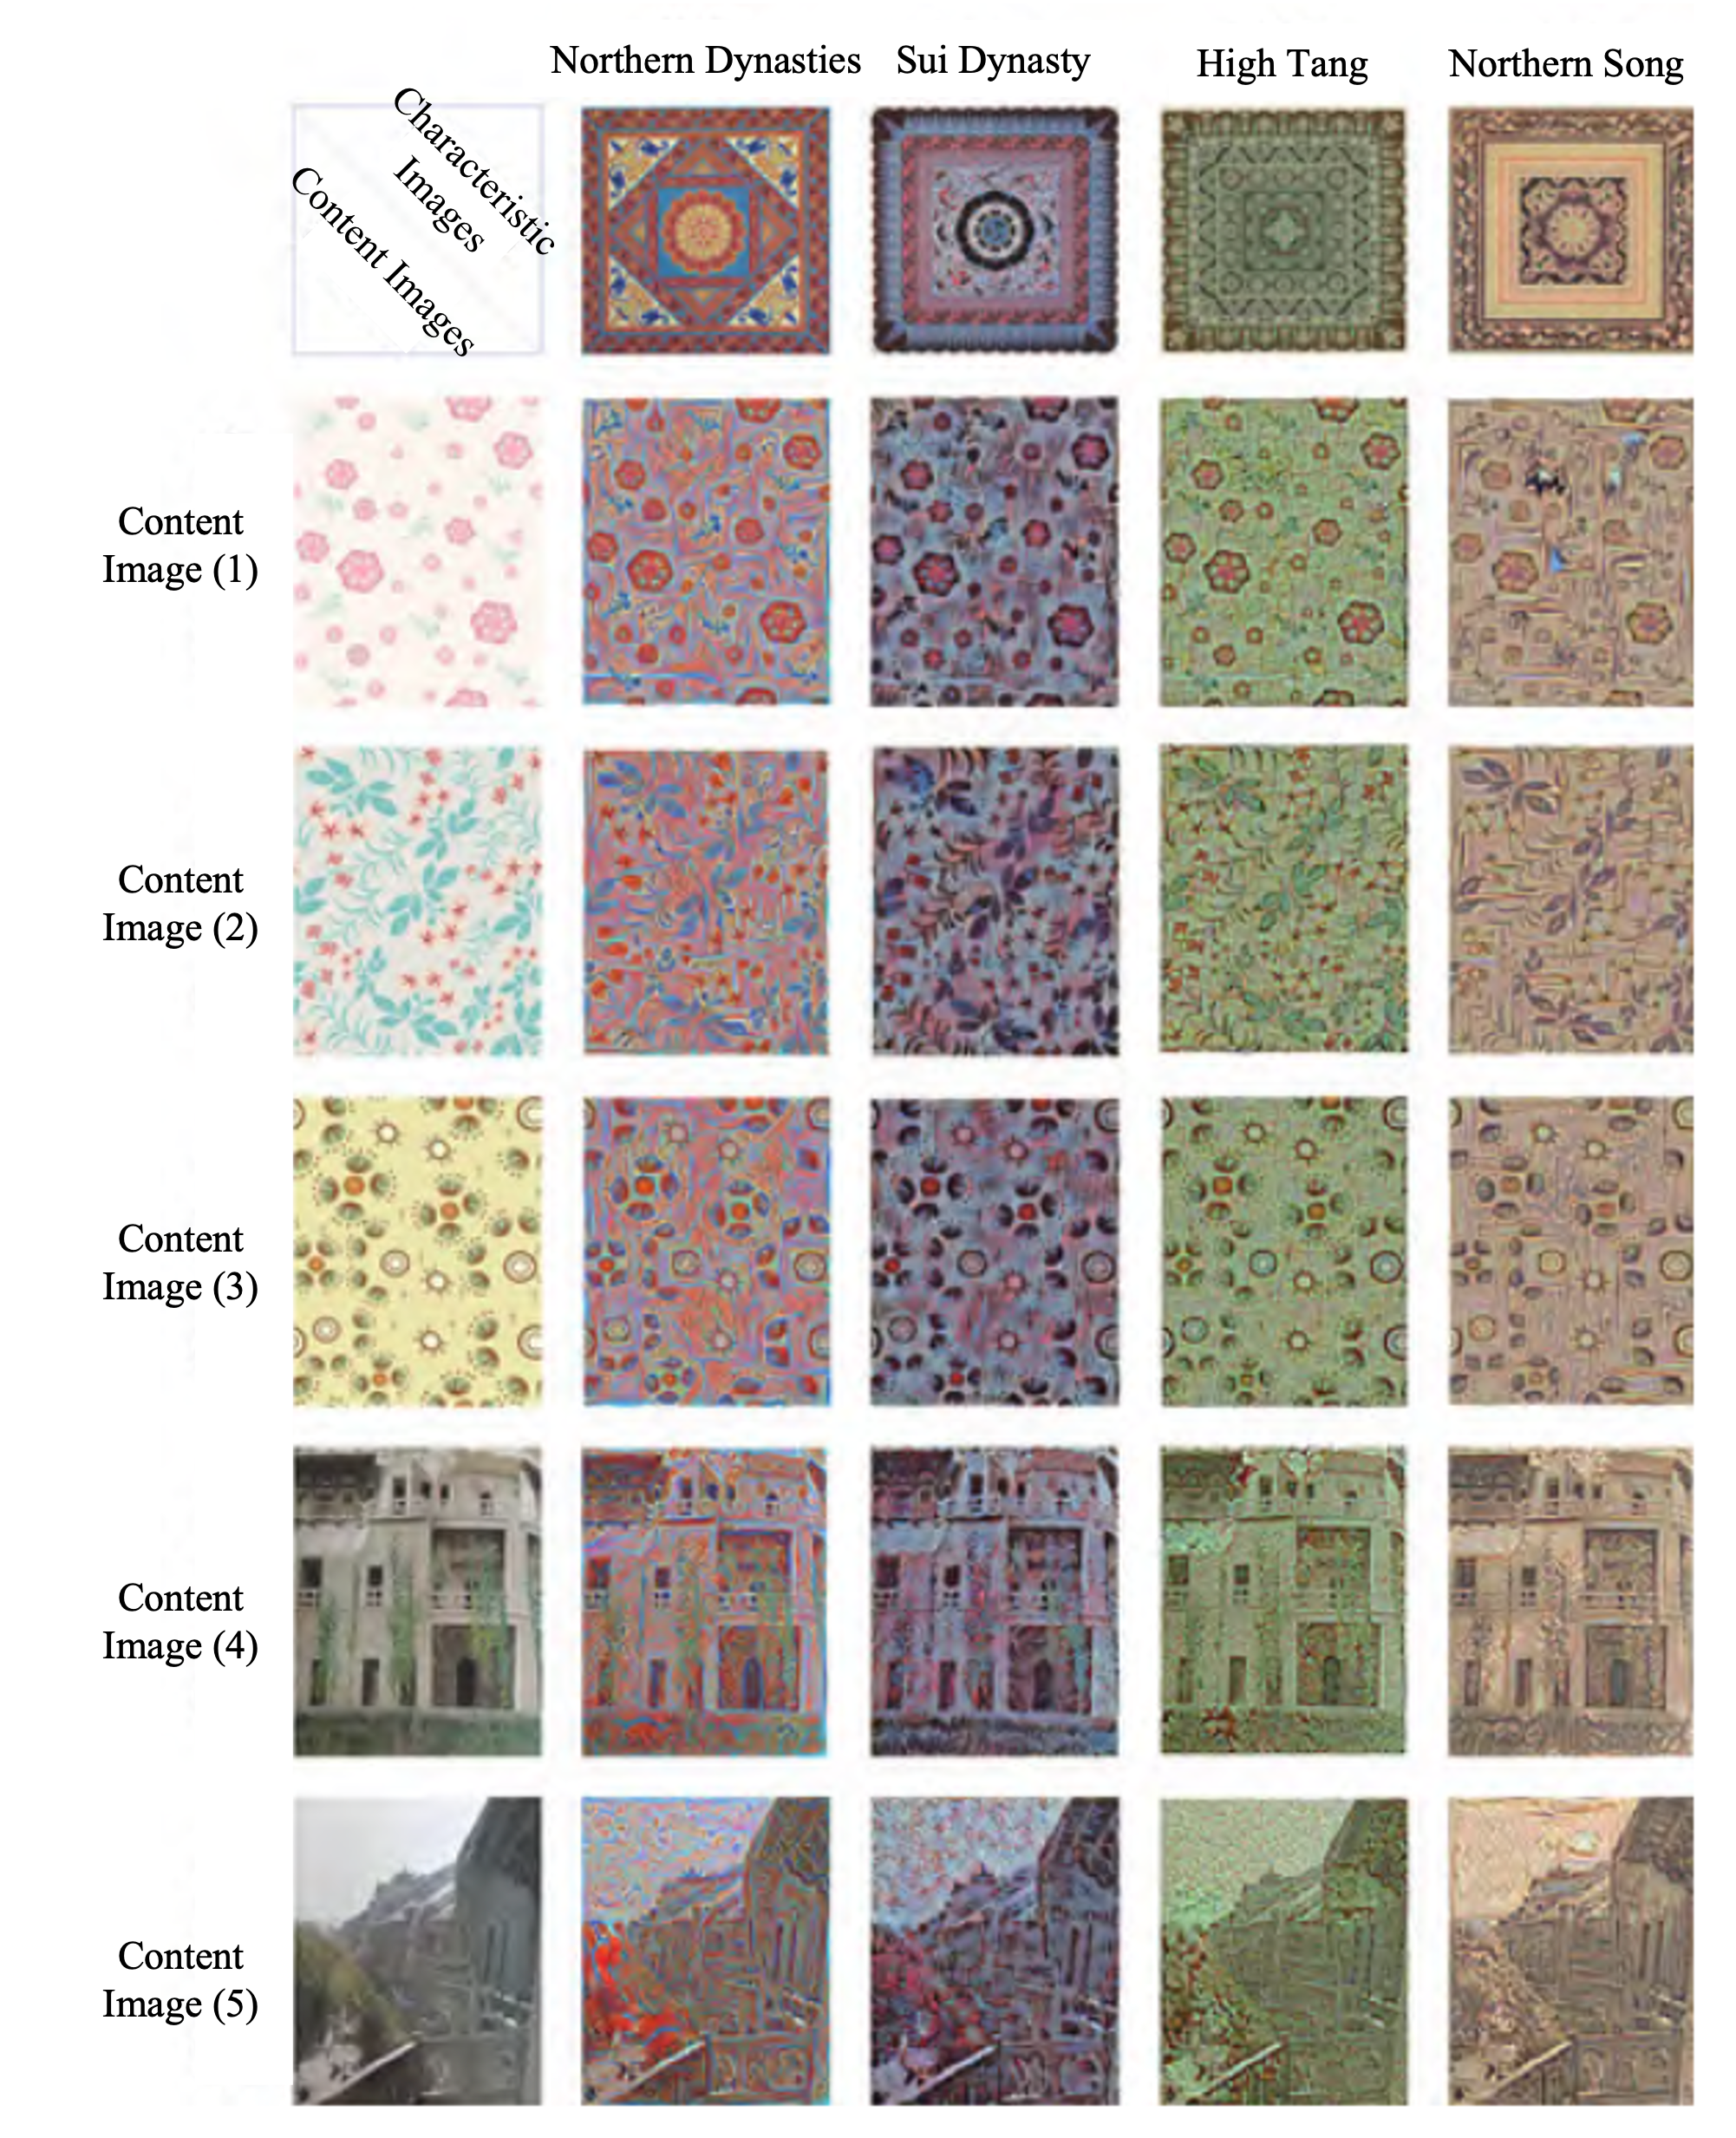
\includegraphics[width=0.9\textwidth]{figs/style-transfer-showcase-en.png}
    \end{center}

    \small\textit{Note.} The original figure were in Chinese. The captions are translted into English
    by the author. \apacitefigfrom{Sun2023-Dunhuang-Patterns}
\end{figure}

\printbibliography